\section{}

Mithilfe des in der Aufgabenstellung geschilderten Vorgehens erhalten wir den folgenden Code:

\lstinputlisting[style=matlabcode, firstline = 1, lastline = 30]{chapter_08/exercise_08_44.m}

Innerhalb weniger Sekunden erhalten wir hieraus das folgende Bild der Mandelbrotmenge:

\begin{center}
  
\includegraphics[width = \textwidth]{chapter_08/exercise_08_44_figure_1.pdf}
\end{center}

Durch Ändern der Parameter (man betrachte die im Quellcode auskommentierten Zeilen) und mehr Rendering-Zeit lässt sich die Mandelbrotmenge nun in verschiedenen Bereichen mit unterschiedlichen Auflösungen und Farbverläufen betrachten:

\begin{center}
  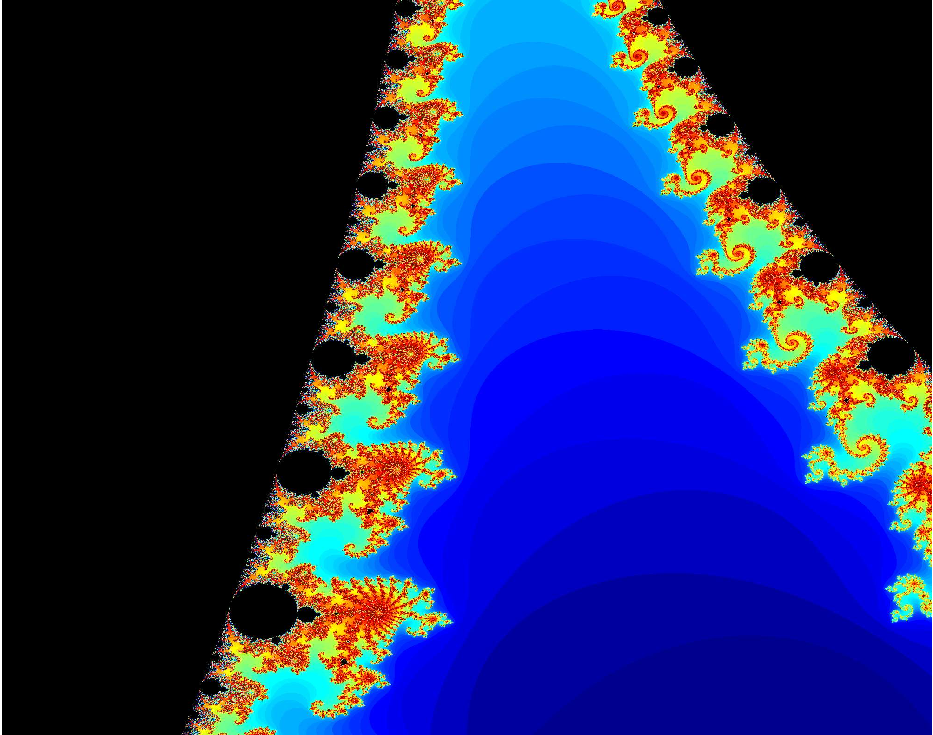
\includegraphics[width = \textwidth]{chapter_08/exercise_08_44_figure_2.pdf}
\end{center}
